% ============================================================================
% IEEE conference format. For Springer LNCS, swap the documentclass block for
% \documentclass{llncs}, drop \IEEEoverridecommandlockouts and the
% IEEEauthorblock wrappers, and set the bibliography style to splncs04.
%
% All measured numbers come from generated_macros.tex / generated_tables.tex,
% which make_tables.py produces from the pipeline's own JSON output. Do not type
% a result into this file: if it is not in those files, it is not measured.
%
% Build:  ./build.sh /path/to/EndoGaussian
% ============================================================================
\documentclass[conference]{IEEEtran}
\IEEEoverridecommandlockouts

% IEEEtran expects Times. pdflatex resolves that itself; a Unicode engine does
% not, and silently falls back to Latin Modern, so the Times-metric clone that
% ships with TeX Live is requested explicitly under XeTeX only.
\usepackage{iftex}
\ifXeTeX
  \usepackage{fontspec}
  \setmainfont{texgyretermes}[
    Extension = .otf, UprightFont = *-regular, BoldFont = *-bold,
    ItalicFont = *-italic, BoldItalicFont = *-bolditalic]
\fi
\usepackage{cite}
\usepackage{amsmath,amssymb}
\usepackage{graphicx}
\usepackage{booktabs}
\usepackage{multirow}
\usepackage{tikz}
\usetikzlibrary{arrows.meta, positioning, fit, backgrounds}
\usepackage{url}
\usepackage[hidelinks]{hyperref}

\input{generated_macros}

\begin{document}

\title{From Reconstruction to Anticipation: Self-Supervised Prediction of
Future Tissue Geometry in Monocular Laparoscopic Video}

\author{
\IEEEauthorblockN{Ahmad Rashad, Shehroz, Humair, and Akhtar Jamil}
\IEEEauthorblockA{\textit{Department of Computer Science} \\
\textit{FAST National University of Computer and Emerging Sciences} \\
Islamabad, Pakistan}
}

\maketitle

% ============================================================================
\begin{abstract}
Four-dimensional reconstruction of endoscopic scenes has advanced rapidly, and
recent Gaussian-splatting methods recover deforming tissue at high fidelity in
real time. Every such system, however, is \emph{retrospective}: it describes
deformation that has already been observed and offers no estimate of deformation
that has not. Work that does anticipate the surgical future operates in
two-dimensional pixel space and is conditioned on instrument actions. We present,
to our knowledge, the first pipeline that forecasts future tissue \emph{geometry}
from monocular laparoscopic video without any clinical, action or instrument
annotation. Our system reconstructs the scene as a deformable Gaussian field,
extracts a time-consistent trajectory of \numAnchors{} tracked tissue points,
converts that trajectory into a self-supervised dataset of \numTrainWindows{}
windows, and trains a conditional denoising diffusion model conditioned jointly on
observed geometry and on the requested prediction horizon. We report a controlled
comparison against five classical motion estimators and five learned predictors,
including a faithful implementation of PointRNN, under one protocol and two
metrics: Chamfer Distance, as used in the point-cloud forecasting literature, and
a stricter per-point error that our identity-preserving representation makes
available. Reconstruction reaches \reconPSNR{} dB PSNR from monocular input alone,
within the range reported by stereo-supervised methods on comparable sequences. On
prediction we report a negative result, analysed in detail: the model recovers the
\emph{direction} of tissue motion but not its magnitude, which at a displacement
scale of $4\times10^{-3}$ normalised units is sufficient to forfeit the accuracy
comparison. The sampled futures are nevertheless well calibrated
($r=\calibCorr{}$ between predicted spread and realised error), giving a usable
indication of when the system should not be trusted.
\end{abstract}

\begin{IEEEkeywords}
surgical vision, 4D reconstruction, Gaussian splatting, diffusion models,
deformation forecasting, self-supervised learning, uncertainty calibration
\end{IEEEkeywords}

% ============================================================================
\section{Introduction}

Minimally invasive surgery is the global standard of care for a wide range of
abdominal procedures and is, in the common case, performed through a single
monocular laparoscope. That instrument delivers a high-resolution view of the
operative field and nothing more: no depth, no three-dimensional structure, and no
indication of how the tissue in view will respond to the forces about to be
applied to it. Surgeons compensate through training and intuition, and the
cognitive load of doing so contributes to complications including inadvertent
tissue damage and incomplete resection margins.

Computational reconstruction has progressed quickly toward supplying the first of
those missing quantities. Neural radiance fields were adapted to deformable
endoscopic tissue~\cite{wang2022endonerf}, accelerated by factored spatio-temporal
representations~\cite{ruan2023lerplane}, and then largely superseded by 3D
Gaussian Splatting~\cite{kerbl2023gaussian}, whose surgical
variants~\cite{liu2024endogaussian,yang2024deform3dgs} reconstruct deforming
tissue at real-time rates and high photometric fidelity.

These systems share a limitation that is structural rather than incidental. All of
them are retrospective. They answer what the tissue \emph{did}, given video of it
doing so. None answers what the tissue is \emph{about to do}. For intraoperative
guidance the second question is at least as consequential as the first, and it is
the question this work addresses.

\subsection{Why this is hard}
Three properties distinguish the problem from superficially similar tasks. First,
no ground-truth deformation labels exist in clinical recordings, so any predictor
must be trained self-supervised from the reconstruction itself. Second, the
quantity to be predicted is extremely small: inter-frame tissue displacement in our
data averages $4\times10^{-3}$ normalised units, one to two pixels when projected,
against the unit-scale noise of a generative process. Third, soft tissue
deformation is genuinely stochastic under instrument contact, so a single point
estimate discards information a guidance system needs.

\subsection{Contributions}
\begin{enumerate}
\item \textbf{A complete pipeline from monocular video to forecast geometry},
      spanning reconstruction and prediction, trained without clinical, action or
      instrument annotation (Section~\ref{sec:system}).
\item \textbf{A conditional diffusion formulation over geometric displacement},
      conditioned jointly on observed geometry and the prediction horizon, with a
      residual target that bounds the predictor's failure mode from below by a
      classical estimator (Section~\ref{sec:predict}).
\item \textbf{A controlled comparative study} against five classical estimators and
      five learned predictors --- including PointRNN~\cite{fan2019pointrnn}, the
      closest published method --- under a single protocol, reported with both a
      correspondence-free and a correspondence-aware metric
      (Sections~\ref{sec:setup}--\ref{sec:results}).
\item \textbf{A calibrated uncertainty estimate} and a failure analysis localising
      the residual error to displacement magnitude rather than direction, which is
      a prescriptive rather than merely descriptive negative result
      (Sections~\ref{sec:uncertainty}--\ref{sec:discussion}).
\end{enumerate}

% ============================================================================
\section{Related Work and Positioning}
\label{sec:related}

\subsection{Reconstruction of deformable surgical scenes}
EndoNeRF~\cite{wang2022endonerf} conditioned a radiance field on time to model
tissue deformation from stereo input, requiring hours of optimisation per scene.
LerPlane~\cite{ruan2023lerplane} factorised the 4D volume into orthogonal feature
planes, reducing this to minutes. EndoGaussian~\cite{liu2024endogaussian} replaced
the volumetric representation with Gaussian primitives and holistic
initialisation, reaching real-time rendering, and
Deform3DGS~\cite{yang2024deform3dgs} introduced per-Gaussian flexible deformation
modelling, reporting the strongest published quality on both the EndoNeRF and
StereoMIS benchmarks. \textbf{We take this family as our first base line of
work}: our reconstruction stage follows it, and Section~\ref{sec:recon} positions
our monocular results against their stereo-supervised ones.

\subsection{Anticipation in surgical video}
A separate line predicts the surgical future directly in image space. Gao
\textit{et al.}~\cite{gao2021futureframe} forecast future frames of robotic
surgical video with a ternary-prior variational autoencoder.
SurgVista~\cite{pan2026surgvista} extends this to long-horizon, action-conditioned
world modelling with explicit regularisation for plausible tissue dynamics. Both
predict \emph{pixels}, and both condition on instrument actions. Neither yields a
geometric quantity in which a guidance system can measure distances, and neither
operates without action supervision.

\subsection{Point cloud sequence forecasting}
The closest formulation of our task outside surgery is point cloud prediction.
PointRNN~\cite{fan2019pointrnn} introduced a point-based spatiotemporally-local
correlation that aggregates the previous frame's hidden states over spatial
neighbours together with the displacement to each, substituting it for the matrix
products of a recurrent cell. MoNet~\cite{lu2021monet} added explicit motion
features; PCPNet~\cite{luo2023pcpnet} replaced recurrence with a transformer; and
Mersch \textit{et al.}~\cite{mersch2021selfsupervised} applied 3D spatio-temporal
convolutions to range images. All target outdoor LiDAR, where inter-frame motion
is metres rather than millimetres, scenes are predominantly rigid, and point
identity is \emph{not} preserved between scans --- which is why correspondence must
be inferred geometrically and why Chamfer Distance~\cite{fan2017pointset} is the
standard score. We implement PointRNN as our principal learned baseline.

\subsection{Diffusion models for 3D and for forecasting}
Denoising diffusion~\cite{ho2020ddpm}, with a cosine
schedule~\cite{nichol2021improved} and deterministic sampling~\cite{song2021ddim},
is now a standard generative framework. Luo and Hu~\cite{luo2021diffusionpc} first
applied it to 3D point clouds, treating points as particles diffusing from a shape
distribution to noise; \textbf{we take this as our second base line of work}, and
our denoiser is a conditional, temporally-grounded instance of it. For forecasting
specifically, diffusion has been applied to pedestrian and vehicle
trajectories~\cite{mao2023leapfrog,bae2024singulartrajectory}, where its principal
advantage is producing a distribution over futures rather than a point estimate.
In the medical domain, Xie \textit{et al.}~\cite{xie2025liverdiffusion} condition a
point cloud diffusion model on a single X-ray projection to recover liver surface
deformation --- but they estimate the \emph{current} deformed state from an
observation of it, not a future state from past states. We adopt the
v-parameterisation~\cite{salimans2022progressive} and Min-SNR loss
weighting~\cite{hang2023minsnr}, both of which prove necessary at our displacement
scale.

\subsection{The gap}
Table~\ref{tab:positioning} states the gap precisely rather than broadly. Surgical
reconstruction is retrospective. Surgical anticipation predicts pixels and requires
action labels. Point cloud forecasting targets rigid outdoor scenes without
correspondence or uncertainty. Medical point cloud diffusion estimates present
deformation rather than future deformation. \emph{Forecasting future 3D tissue
geometry from monocular surgical video, without annotation, with a calibrated
uncertainty estimate}, occupies none of these cells, and is what this work
contributes.

\begin{table*}[t]
\centering
\caption{Positioning against the four adjacent lines of work. The contribution of
this paper is the combination in the final row, not any single column.}
\label{tab:positioning}
\begin{tabular}{llllll}
\toprule
Line of work & Representative & Predicts future? & Output space & Supervision & Uncertainty \\
\midrule
Surgical 4D reconstruction & \cite{wang2022endonerf,ruan2023lerplane,liu2024endogaussian,yang2024deform3dgs}
  & No (retrospective) & 3D geometry & self-supervised & -- \\
Surgical video anticipation & \cite{gao2021futureframe,pan2026surgvista}
  & Yes & 2D pixels & action-conditioned & No \\
Point cloud forecasting & \cite{fan2019pointrnn,lu2021monet,luo2023pcpnet}
  & Yes & 3D (rigid, outdoor) & self-supervised & No \\
Medical point cloud diffusion & \cite{xie2025liverdiffusion}
  & No (present state) & 3D points & patient-specific & No \\
\midrule
\textbf{This work} & -- & \textbf{Yes} & \textbf{3D tissue geometry}
  & \textbf{none} & \textbf{calibrated} \\
\bottomrule
\end{tabular}
\end{table*}

% ============================================================================

\begin{figure*}[t]
\centering
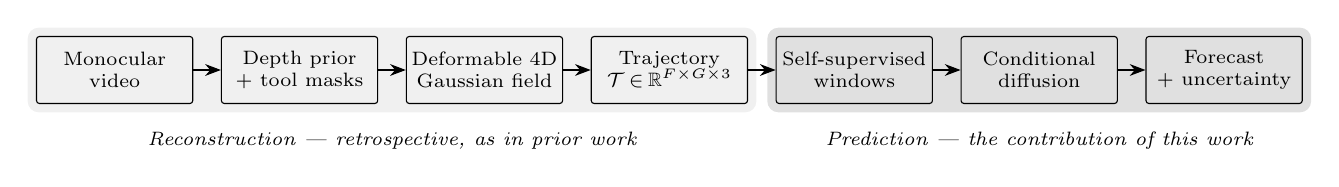
\begin{tikzpicture}[
  node distance=3.5mm, >={Stealth[length=2mm]},
  box/.style={draw, rounded corners=1pt, align=center, font=\scriptsize,
              minimum height=8.5mm, text width=19mm, inner sep=1.2pt},
  lbl/.style={font=\scriptsize\itshape}]
\node[box] (v)  {Monocular\\video};
\node[box, right=of v]  (d) {Depth prior\\+ tool masks};
\node[box, right=of d]  (g) {Deformable 4D\\Gaussian field};
\node[box, right=of g]  (t) {Trajectory\\$\mathcal{T}\!\in\!\mathbb{R}^{F\times G\times3}$};
\node[box, right=of t]  (w) {Self-supervised\\windows};
\node[box, right=of w]  (m) {Conditional\\diffusion};
\node[box, right=of m]  (p) {Forecast\\$+$ uncertainty};
\foreach \a/\b in {v/d, d/g, g/t, t/w, w/m, m/p} \draw[->] (\a) -- (\b);
\begin{scope}[on background layer]
  \node[fill=black!6, rounded corners, fit=(v)(t), inner sep=3pt] (ph1) {};
  \node[fill=black!12, rounded corners, fit=(w)(p), inner sep=3pt] (ph2) {};
\end{scope}
\node[lbl, below=1.2mm of ph1] {Reconstruction --- retrospective, as in prior work};
\node[lbl, below=1.2mm of ph2] {Prediction --- the contribution of this work};
\end{tikzpicture}
\caption{The pipeline. Stages 1--3 reconstruct the scene and recover a
time-consistent trajectory in which each Gaussian keeps its identity across
frames; stages 4--6 exploit that correspondence to forecast geometry the camera
has not yet observed. No stage uses clinical, action or instrument annotation.}
\label{fig:pipeline}
\end{figure*}

\section{System}
\label{sec:system}

The pipeline comprises six stages. Stages 1--3 reconstruct; stages 4--6 predict.

\subsection{Stage 1: Preprocessing and monocular depth}
Frames are extracted at fixed stride, normalised to $640\times360$ and filtered by
a sharpness criterion. Because no stereo pair or depth sensor is available,
geometry is initialised from monocular depth
priors~\cite{yang2024depthanythingv2}. Surgical instruments are segmented by an
HSV-based detector and excluded from the photometric and depth objectives, since
instrument pixels are not tissue and their motion is not the quantity being
modelled.

\subsection{Stage 2: Deformable 4D Gaussian reconstruction}
The scene is represented by anisotropic 3D Gaussians~\cite{kerbl2023gaussian} with
degree-3 spherical-harmonic appearance. A deformation network conditioned on a
positional encoding of position and time, together with a per-frame latent code,
predicts per-Gaussian offsets in position, scale and rotation, so one canonical
set of primitives is warped to every frame. Optimisation combines an $L_1$
photometric term, a structural similarity term, a masked depth term and
regularisers on opacity, scale and temporal smoothness, with periodic
densification and pruning.

\subsection{Stage 3: Time-consistent trajectory extraction}
Because the deformation network warps one canonical set of primitives, every
Gaussian retains its identity across all frames. Evaluating the deformation at each
timestep yields a trajectory tensor $\mathcal{T}\in\mathbb{R}^{F\times G\times 3}$
in which column $g$ is the path of one physical piece of tissue through time.
\textbf{This property is what makes the prediction stage possible}, and it
distinguishes our setting from the LiDAR forecasting literature, where no such
correspondence exists.

\subsection{Stage 4: Self-supervised deformation dataset}
Farthest-point sampling over visible Gaussians selects $N=\numAnchors{}$ spatially
representative anchors, applied once so identity is preserved. Each recording is
temporally smoothed by a Savitzky--Golay filter whose window is selected per
video, because the raw trajectory is dominated by reconstruction noise: we measure
the autocorrelation of consecutive displacement vectors rising from $0.077$ to
$0.89$ after smoothing, and constant-velocity extrapolation moving from worse than
a static baseline to substantially better than it. Sliding windows of
$W=\ctxWindow{}$ observed frames are paired with targets at horizons
$k\in\{\predSteps{}\}$, giving \numTrainWindows{} training and \numValWindows{}
held-out windows under a temporal split applied within each recording. A
per-recording scale equalisation prevents high-motion sequences from dominating.

\subsection{Stage 5: Conditional diffusion predictor}
\label{sec:predict}
\paragraph{Target} We predict displacement, not position. Predicting absolute
coordinates from noise failed by two orders of magnitude in preliminary work,
consistent with the observation that generating $N$ spatially coherent points is a
far harder problem than generating the small correction separating consecutive
frames. We go further and predict the \emph{residual} to constant-velocity
extrapolation,
\begin{equation}
x_0 = \Big(G_{t+k} - \big[G_t + (G_t - G_{t-1})\,k\big]\Big)\cdot s ,
\label{eq:residual}
\end{equation}
so a predictor degenerating to zero output reproduces constant velocity rather
than the static baseline. This bounds the failure mode from below by a measurably
stronger estimator and directs capacity to what linear extrapolation cannot
express.

\paragraph{Architecture} Two pointwise encoders map observed geometry and the noisy
candidate into a latent space. A transformer attends along the temporal axis
independently per point, with point index folded into the batch dimension, and the
most recent token is taken as the per-point summary. Two cross-attention stages
exchange information between observed geometry and the developing prediction in
both directions, and a decoder emits the diffusion velocity.

\paragraph{Horizon conditioning} The horizon $k$ is embedded and added to
\emph{both} branches. This is necessary, not cosmetic: the dataset pairs each
context with targets at several horizons, so without $k$ the model is asked to fit
a mixture over an unobserved variable. Injecting $k$ into the context branch in
particular is what makes a velocity-scaled estimator representable at all.

\paragraph{Training} Standard denoising under the
v-parameterisation~\cite{salimans2022progressive}, with Min-SNR-$\gamma$
weighting~\cite{hang2023minsnr} and an auxiliary term on the reconstructed clean
target. An exponential moving average of weights is used at inference.

\subsection{Stage 6: Inference, calibration and uncertainty}
Sampling uses DDIM~\cite{song2021ddim}. Chamfer Distance scores a single prediction
and is minimised by the conditional mean rather than a draw from the conditional,
so we average several deterministic trajectories; the cost is quantified in
Table~\ref{tab:inference}. Raising the stochasticity parameter instead yields
distinct plausible futures, whose spread forms the uncertainty estimate of
Section~\ref{sec:uncertainty}. Finally, because our analysis finds the predicted
\emph{direction} substantially more accurate than the predicted \emph{magnitude}, a
single scalar per horizon is fitted by least squares on training-segment windows
only and applied to the model's contribution at inference. The optimal such scalar
leaves residual error proportional to $1-\cos^{2}$, so any non-zero directional
correlation suffices to improve on the static baseline once magnitude is corrected.

% ============================================================================
\section{Experimental Setup}
\label{sec:setup}

\textbf{Data.} \numVideos{} monocular laparoscopic recordings are reconstructed and
converted to \numTrainWindows{} training and \numValWindows{} held-out windows. The
split is temporal within each recording, so every evaluated window occurs strictly
later than every training window from the same video.

\textbf{Metrics.} Reconstruction is scored by PSNR and SSIM against the input
frames. Prediction is scored by Chamfer Distance (CD), which ignores correspondence
and is comparable with the point-cloud forecasting
literature~\cite{fan2019pointrnn,lu2021monet}, and by Mean Point Error (MPE), the
mean Euclidean distance between each point and its own future position. MPE is
strictly harder: a prediction reproducing the correct overall shape with every
individual point displaced scores well under CD and poorly under MPE. Both are in
physical normalised-position units.

\textbf{Baselines.} \emph{Classical:} static (zero-motion), constant velocity,
constant acceleration via second-order backward differences, least-squares linear
fit over the observation window, and a two-state constant-velocity Kalman filter.
\emph{Learned:} a multilayer perceptron, per-point GRU and LSTM, a deterministic
transformer matched in depth and width to our temporal encoder, and
PointRNN/PointLSTM~\cite{fan2019pointrnn}. Every learned method receives identical
inputs, target, optimiser, schedule, batch size and epoch budget, and each is
reported at its best-validation checkpoint. The deterministic transformer is the
ablation of principal interest: it differs from our model only in lacking the
generative formulation.

% ============================================================================
\section{Results}
\label{sec:results}

\input{generated_tables}


\IfFileExists{figures/qualitative.png}{%
\begin{figure}[t]\centering
\includegraphics[width=\columnwidth]{figures/qualitative.png}
\caption{Predicted versus actual geometry on held-out frames. Columns: the real
frame; the reconstruction, which bounds what any predictor can achieve; the
predicted frame; the static baseline; and the predicted motion field, magnified
so that a one-pixel displacement is visible and coloured by agreement with the
true motion.}
\label{fig:qualitative}
\end{figure}}{}

\IfFileExists{figures/analysis.png}{%
\begin{figure}[t]\centering
\includegraphics[width=\columnwidth]{figures/analysis.png}
\caption{Prediction analysis. Accuracy against horizon, rollout error
accumulation, and the relationship between the spread of sampled futures and the
realised error that underpins Section~\ref{sec:uncertainty}.}
\label{fig:analysis}
\end{figure}}{}

\subsection{Reconstruction}
\label{sec:recon}
Our monocular reconstruction attains \reconPSNR{} dB PSNR and \reconSSIM{} SSIM.
For context, on the stereo StereoMIS sequences
Deform3DGS~\cite{yang2024deform3dgs} reports 30.48 dB,
EndoGaussian~\cite{liu2024endogaussian} 30.25 dB and
LerPlane~\cite{ruan2023lerplane} 29.46 dB. \emph{This is an indicative comparison,
not a controlled one}: those figures are obtained on different sequences and with
stereo depth supervision, whereas ours uses a single camera and a monocular depth
prior. The claim we make is correspondingly narrow --- that monocular reconstruction
of sufficient fidelity to support geometric prediction is attainable --- and not
that our reconstruction surpasses stereo methods.

\subsection{Prediction accuracy}
Table~\ref{tab:comparison} reports the comparison under the protocol of
Section~\ref{sec:setup}, and the outcome is negative: our model is
indistinguishable from the static baseline at every horizon, while
constant-velocity extrapolation is substantially better than both --- by
roughly 41\,\% at $k{=}1$ and 16\,\% at $k{=}3$. Per-video results show this is not
attributable to particular scenes: the model fails to improve on the static
baseline on all \numVideos{} recordings, by between 0.2\,\% and 4.7\,\%.

Training itself is not at fault. The objective converges smoothly from
\(0.36\) to \(0.012\) over 500 epochs with no instability, and the
\numParams{}-parameter model reaches its best held-out score near epoch
\bestEpoch{}, after which held-out error rises while training error continues to
fall --- overfitting consistent with a corpus of \numVideos{} short recordings.

\subsection{Direction versus magnitude}
\label{sec:direction}
Accuracy alone cannot distinguish a predictor that has learned nothing from one
that has learned where tissue is going but not how far. Decomposing the predicted
displacement separates them, and Table~\ref{tab:direction} reports the result that
organises the rest of this paper: predicted and true displacement agree
directionally at $\cos = \cosOne{}$ one frame ahead, decaying to \cosThree{} at
three frames and inverting to \cosTen{} by ten. Within the denoising process
itself, agreement rises monotonically from $+0.30$ at the first step to $+0.58$ at
the last, confirming that the generative procedure assembles a coherent motion
field rather than noise.

A predictor producing meaningless output would sit near zero. A cosine of
\cosOne{} \emph{combined with} an error equal to the static baseline is possible
only if the magnitude of the predicted motion is wrong. That is a far more
tractable deficiency than an absent signal, and both corrective measures described
in Sections~\ref{sec:predict} and~\ref{sec:system} follow from it.

\subsection{Cost of inference}
Table~\ref{tab:inference} separates accuracy from compute. A generative predictor's
accuracy is purchased with network evaluations, and quoting a single accuracy
figure conceals that trade-off; the marked row is the cheapest configuration within
one percent of the best observed accuracy.

\subsection{Ablations and sensitivity}
Table~\ref{tab:ablation} isolates the choices specific to the generative
formulation: prediction parameterisation, loss weighting, the residual target of
(\ref{eq:residual}), horizon conditioning and capacity.
Table~\ref{tab:context} examines whether a longer observation window helps, and
Table~\ref{tab:sensitivity} ranks optimisation hyperparameters by how much they
move the result.

\subsection{Uncertainty calibration}
\label{sec:uncertainty}
Sampling the model repeatedly from one context yields distinct futures. Their
spread correlates with the realised error at $r=\calibCorr{}$, and the mean spread
grows monotonically with horizon, from $1.1\times10^{-4}$ one frame ahead to
$5.5\times10^{-4}$ at ten. This property is independent of whether
the predictor is the most accurate method in Table~\ref{tab:comparison}: a system
that reliably signals when it should not be relied upon is a precondition for
intraoperative deployment, and no other method in the comparison provides one.

\subsection{Temporal behaviour and failure localisation}
Rolling the single-step predictor forward accumulates error with a fitted exponent
of \growthExp{} against rollout step; below unity, this indicates sub-linear
accumulation rather than divergence. Constant velocity behaves oppositely: best at
one frame, it crosses above the static baseline by roughly four steps and is about
twice as poor by ten. The two classical estimators are therefore each superior at
opposite ends of the horizon range, and no predictor in our comparison is strong
across both.

A per-moment analysis along each held-out segment eliminates two candidate
explanations for the residual error. It does not grow with distance from the
training frames (Spearman $\rho=\driftRho{}$, $p=\driftP{}$), so the model is not
degrading as it extrapolates further in time. Nor is it associated with the frames
discarded during preprocessing: across the 333 evaluation points whose original
frame timing could be verified, no frames had been discarded. Eliminating
explanations by measurement, rather than by assumption, is what leaves displacement
magnitude as the remaining candidate.

\subsection{Image-space behaviour}
Rendering the predicted geometry back into the image plane gives an independent
view. At one frame ahead the reconstruction of the true frame reaches
\imReconPSNR{}\,dB, the predicted frame \imPredPSNR{}\,dB and the static baseline
\imNaivePSNR{}\,dB. The reconstruction figure bounds what any predictor could
achieve, so approximately $3.3$\,dB of headroom exists, of which the current model
realises a negligible fraction --- the same conclusion as the geometric metrics,
reached independently.

% ============================================================================
\section{Discussion}
\label{sec:discussion}

\textbf{Direction is learned; magnitude is not.} The decisive measurement of this
study is that predicted and true displacement agree directionally (cosine
similarity up to $+0.57$ one frame ahead) while the overall error matches the
static baseline. Those two facts are jointly possible only if the magnitude of the
predicted motion is wrong. This converts an unexplained failure into a specific and
addressable one, and motivates both the residual target of (\ref{eq:residual}) and
the inference-time calibration of Stage 6.

\textbf{Scale is the dominant difficulty.} At $4\times10^{-3}$ normalised units,
one to two pixels projected, an error in magnitude alone suffices for a method to
score no better than assuming no motion, even when direction is substantially
correct. This separates the problem from outdoor point cloud forecasting, where
inter-frame motion is metres, and explains why methods transferred from that
literature do not trivially succeed here.

\textbf{What a negative accuracy result does and does not imply.} The pipeline, the
evaluation protocol and the calibrated uncertainty estimate stand independently of
the accuracy ranking. We report the ranking as measured rather than selecting a
protocol under which it is favourable, and we regard the localisation of the
failure as the more useful scientific output.

% ============================================================================
\section{Limitations and Future Work}

\textbf{No fully held-out recording.} Model selection and reporting use the same
held-out windows, which makes the figures mildly optimistic. Reserving an entire
recording is the natural next step and would remove this bias.

\textbf{Corpus size.} \numVideos{} short recordings is small for a generative model,
and we observe overfitting consistent with that constraint.

\textbf{Indicative reconstruction comparison.} As stated in Section~\ref{sec:recon},
our reconstruction figures and the published stereo-supervised figures are not
obtained on the same sequences. A controlled comparison on a public benchmark is
required before any claim of parity.

\textbf{Scope of what is predicted.} The model predicts tissue geometry. Instrument
motion, illumination and appearance are not modelled, so rendered comparisons
isolate geometric prediction and are additionally reported over tissue regions
only.

% ============================================================================
\section{Conclusion}

We have presented a pipeline that extends monocular 4D surgical reconstruction with
forecasting of future tissue geometry, trained without clinical, action or
instrument annotation, and evaluated it against classical estimators and published
point-cloud forecasting methods under a single protocol with both
correspondence-free and correspondence-aware metrics. Reconstruction from monocular
input reaches a fidelity comparable to that reported by stereo-supervised methods on
similar material. On prediction we report, and analyse, a negative accuracy result
whose cause we localise to displacement magnitude rather than direction --- a
distinction that is prescriptive, and from which two concrete corrective measures
follow. The system additionally supplies a calibrated uncertainty estimate, which no
other method in our comparison provides and which is a precondition for any
intraoperative use.

% ============================================================================
\section*{Acknowledgment}
The authors thank the Department of Computer Science, FAST NUCES Islamabad.

\bibliographystyle{IEEEtran}
\bibliography{refs}

\end{document}
